% Auto-generated LaTeX snippet for report figures
% Add \usepackage{graphicx} and \usepackage{float} in your preamble.

\begin{figure}[H]
    \centering
    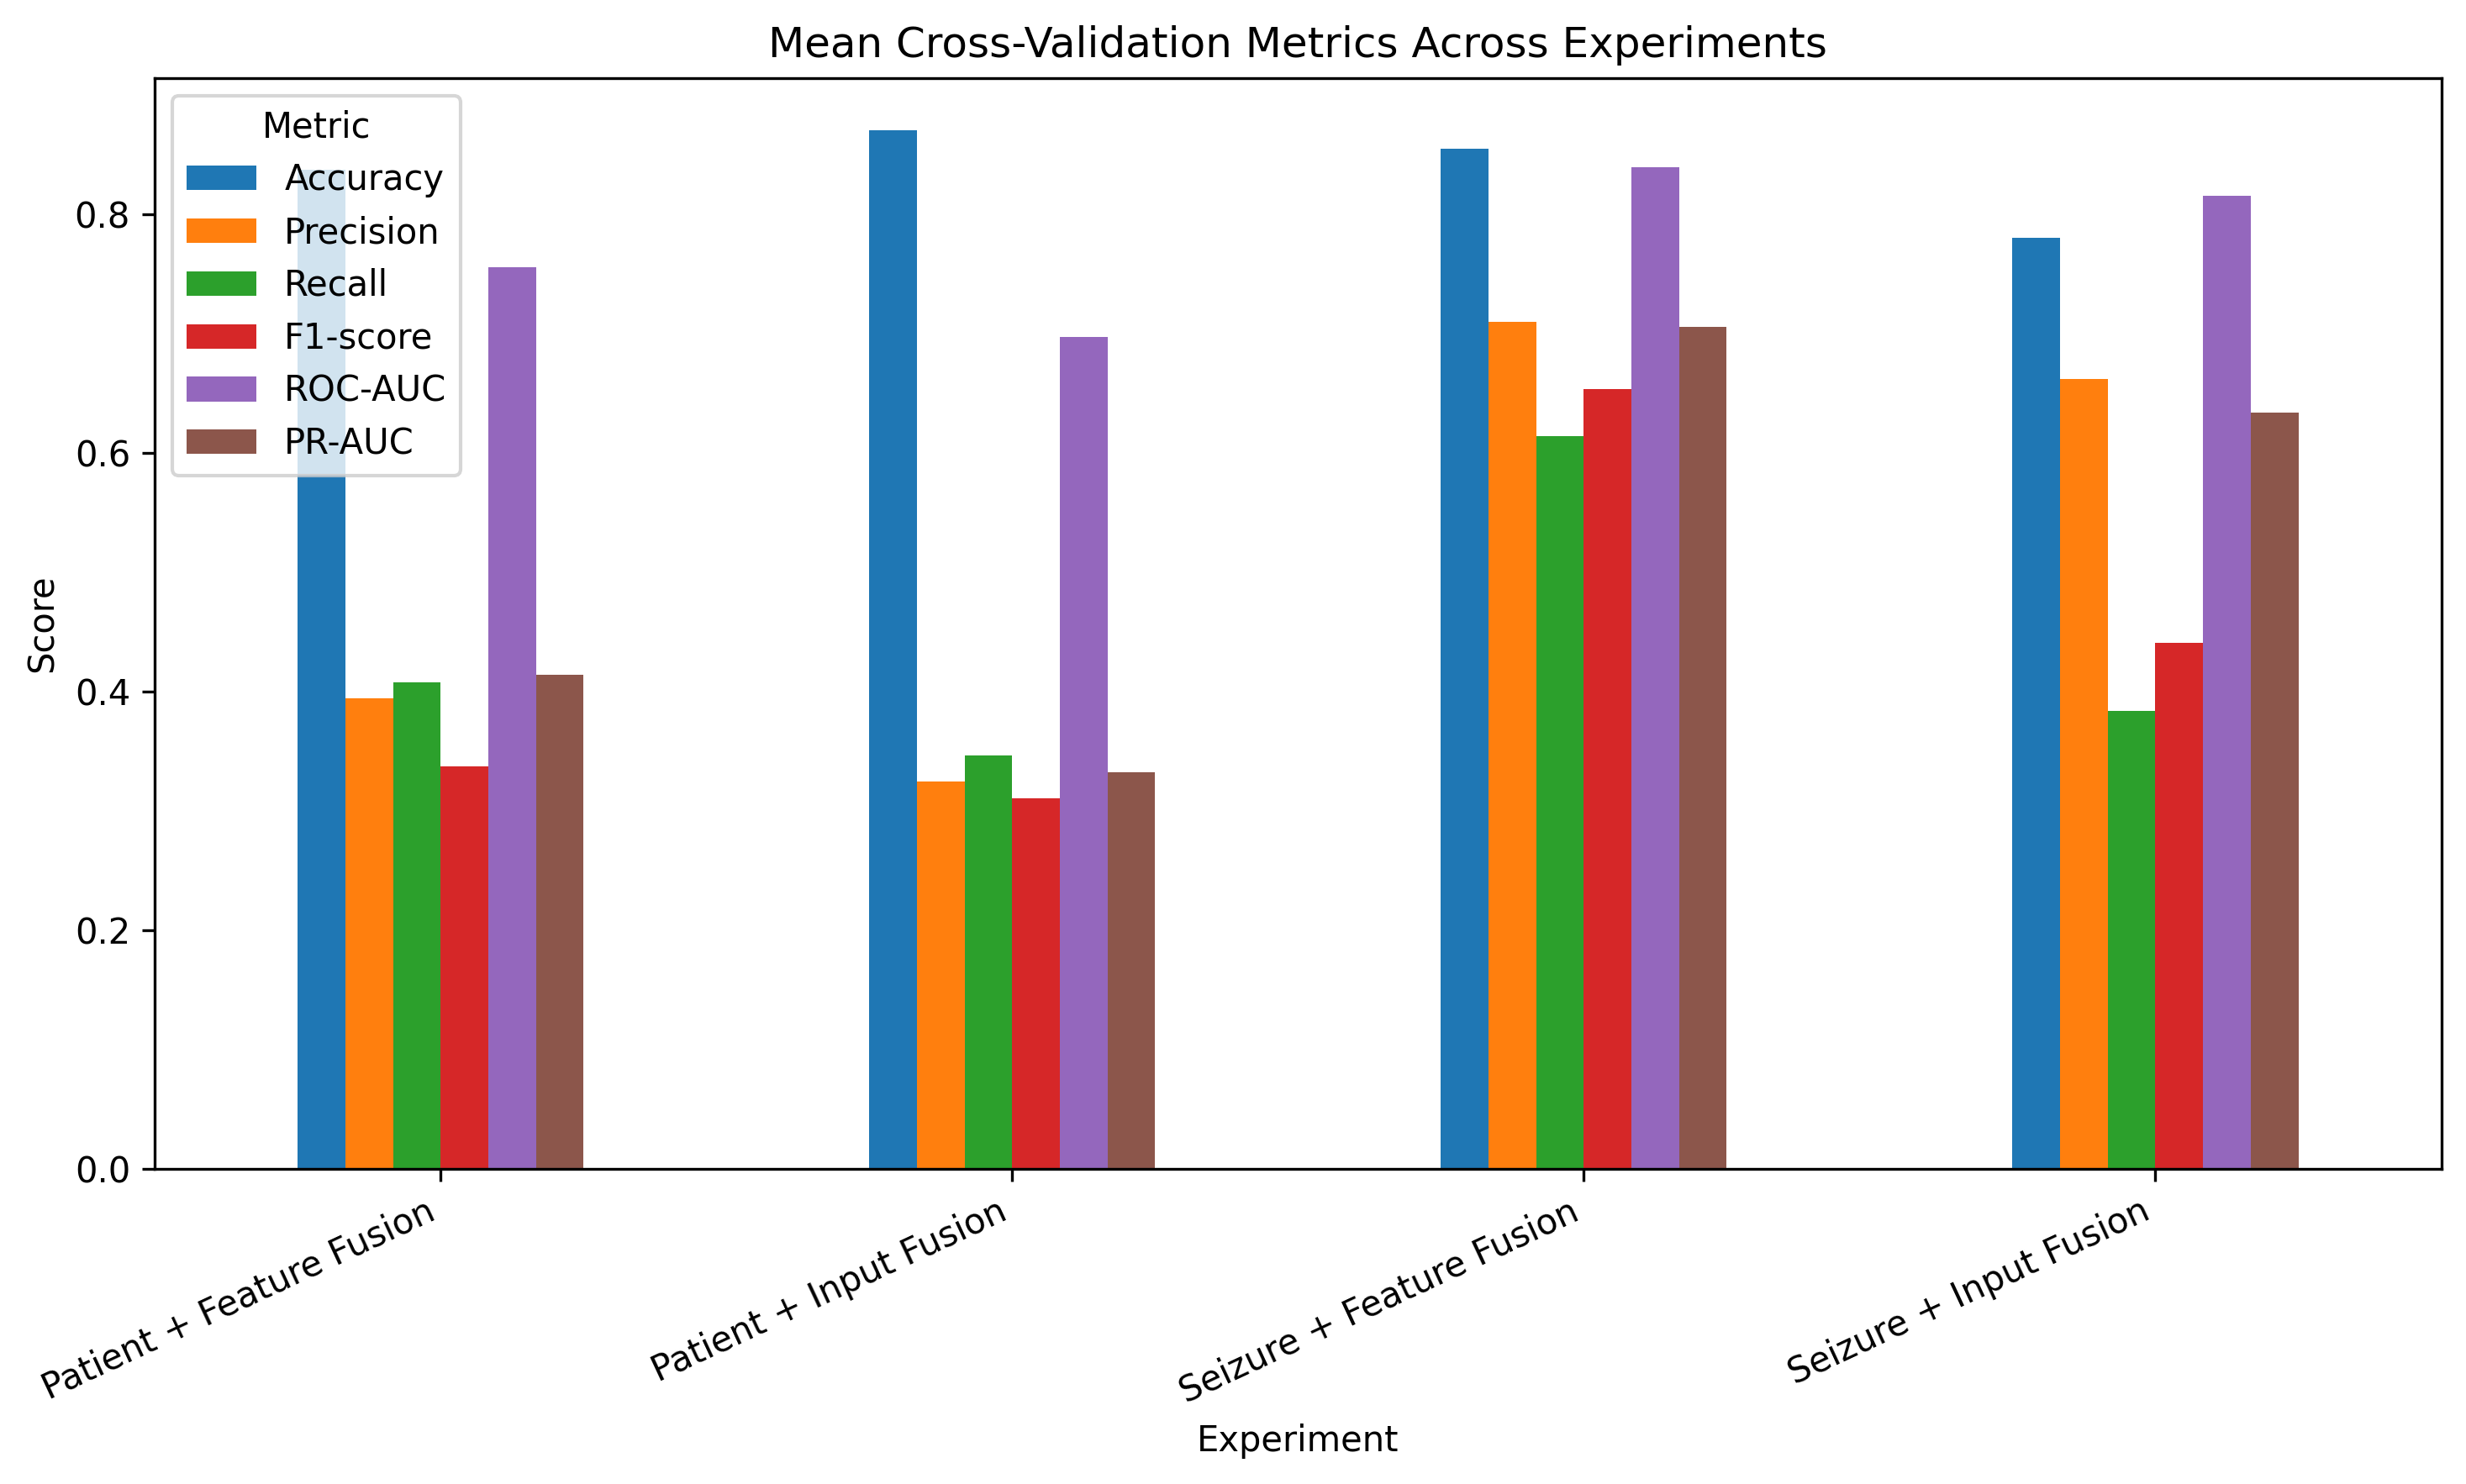
\includegraphics[width=0.88\textwidth]{generated_figures/Fig_01_mean_crossval_metrics.png}
    \caption{Mean cross-validation metrics across the four experiment settings.}
    \label{fig:mean_crossval_metrics}
\end{figure}

\begin{figure}[H]
    \centering
    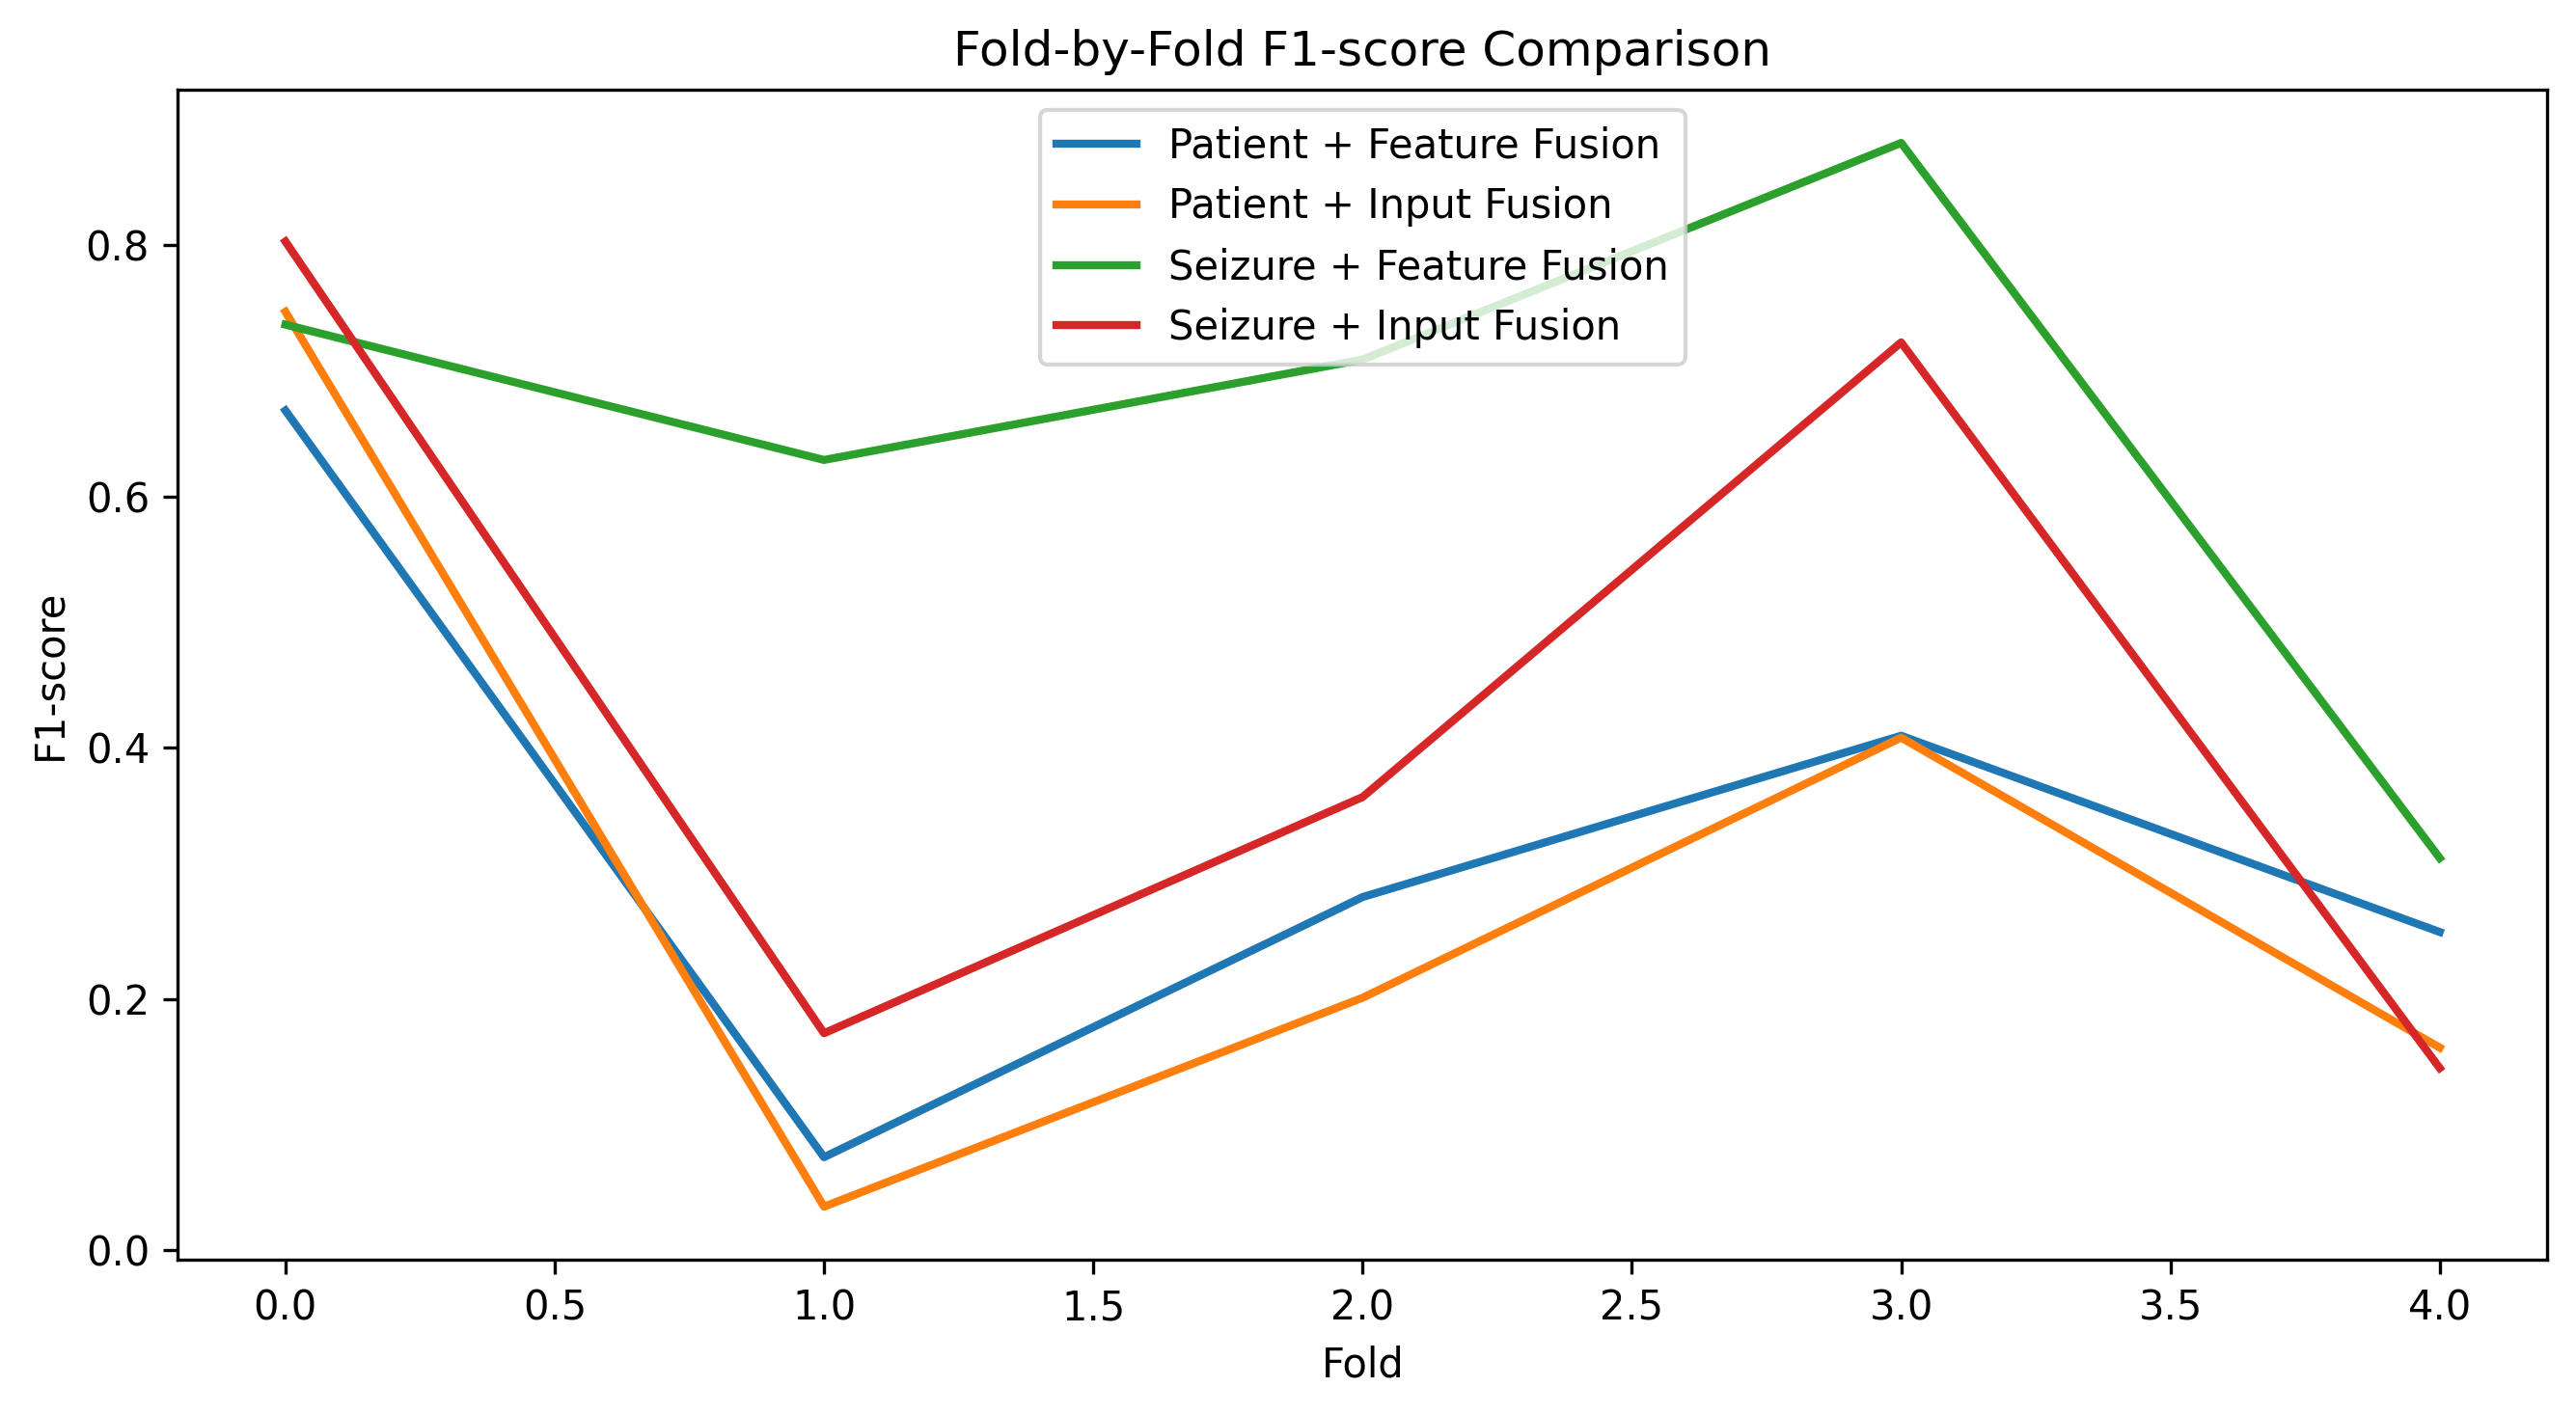
\includegraphics[width=0.88\textwidth]{generated_figures/Fig_02_foldwise_f1.png}
    \caption{Fold-by-fold F1-score comparison across all experiments.}
    \label{fig:foldwise_f1}
\end{figure}

\begin{figure}[H]
    \centering
    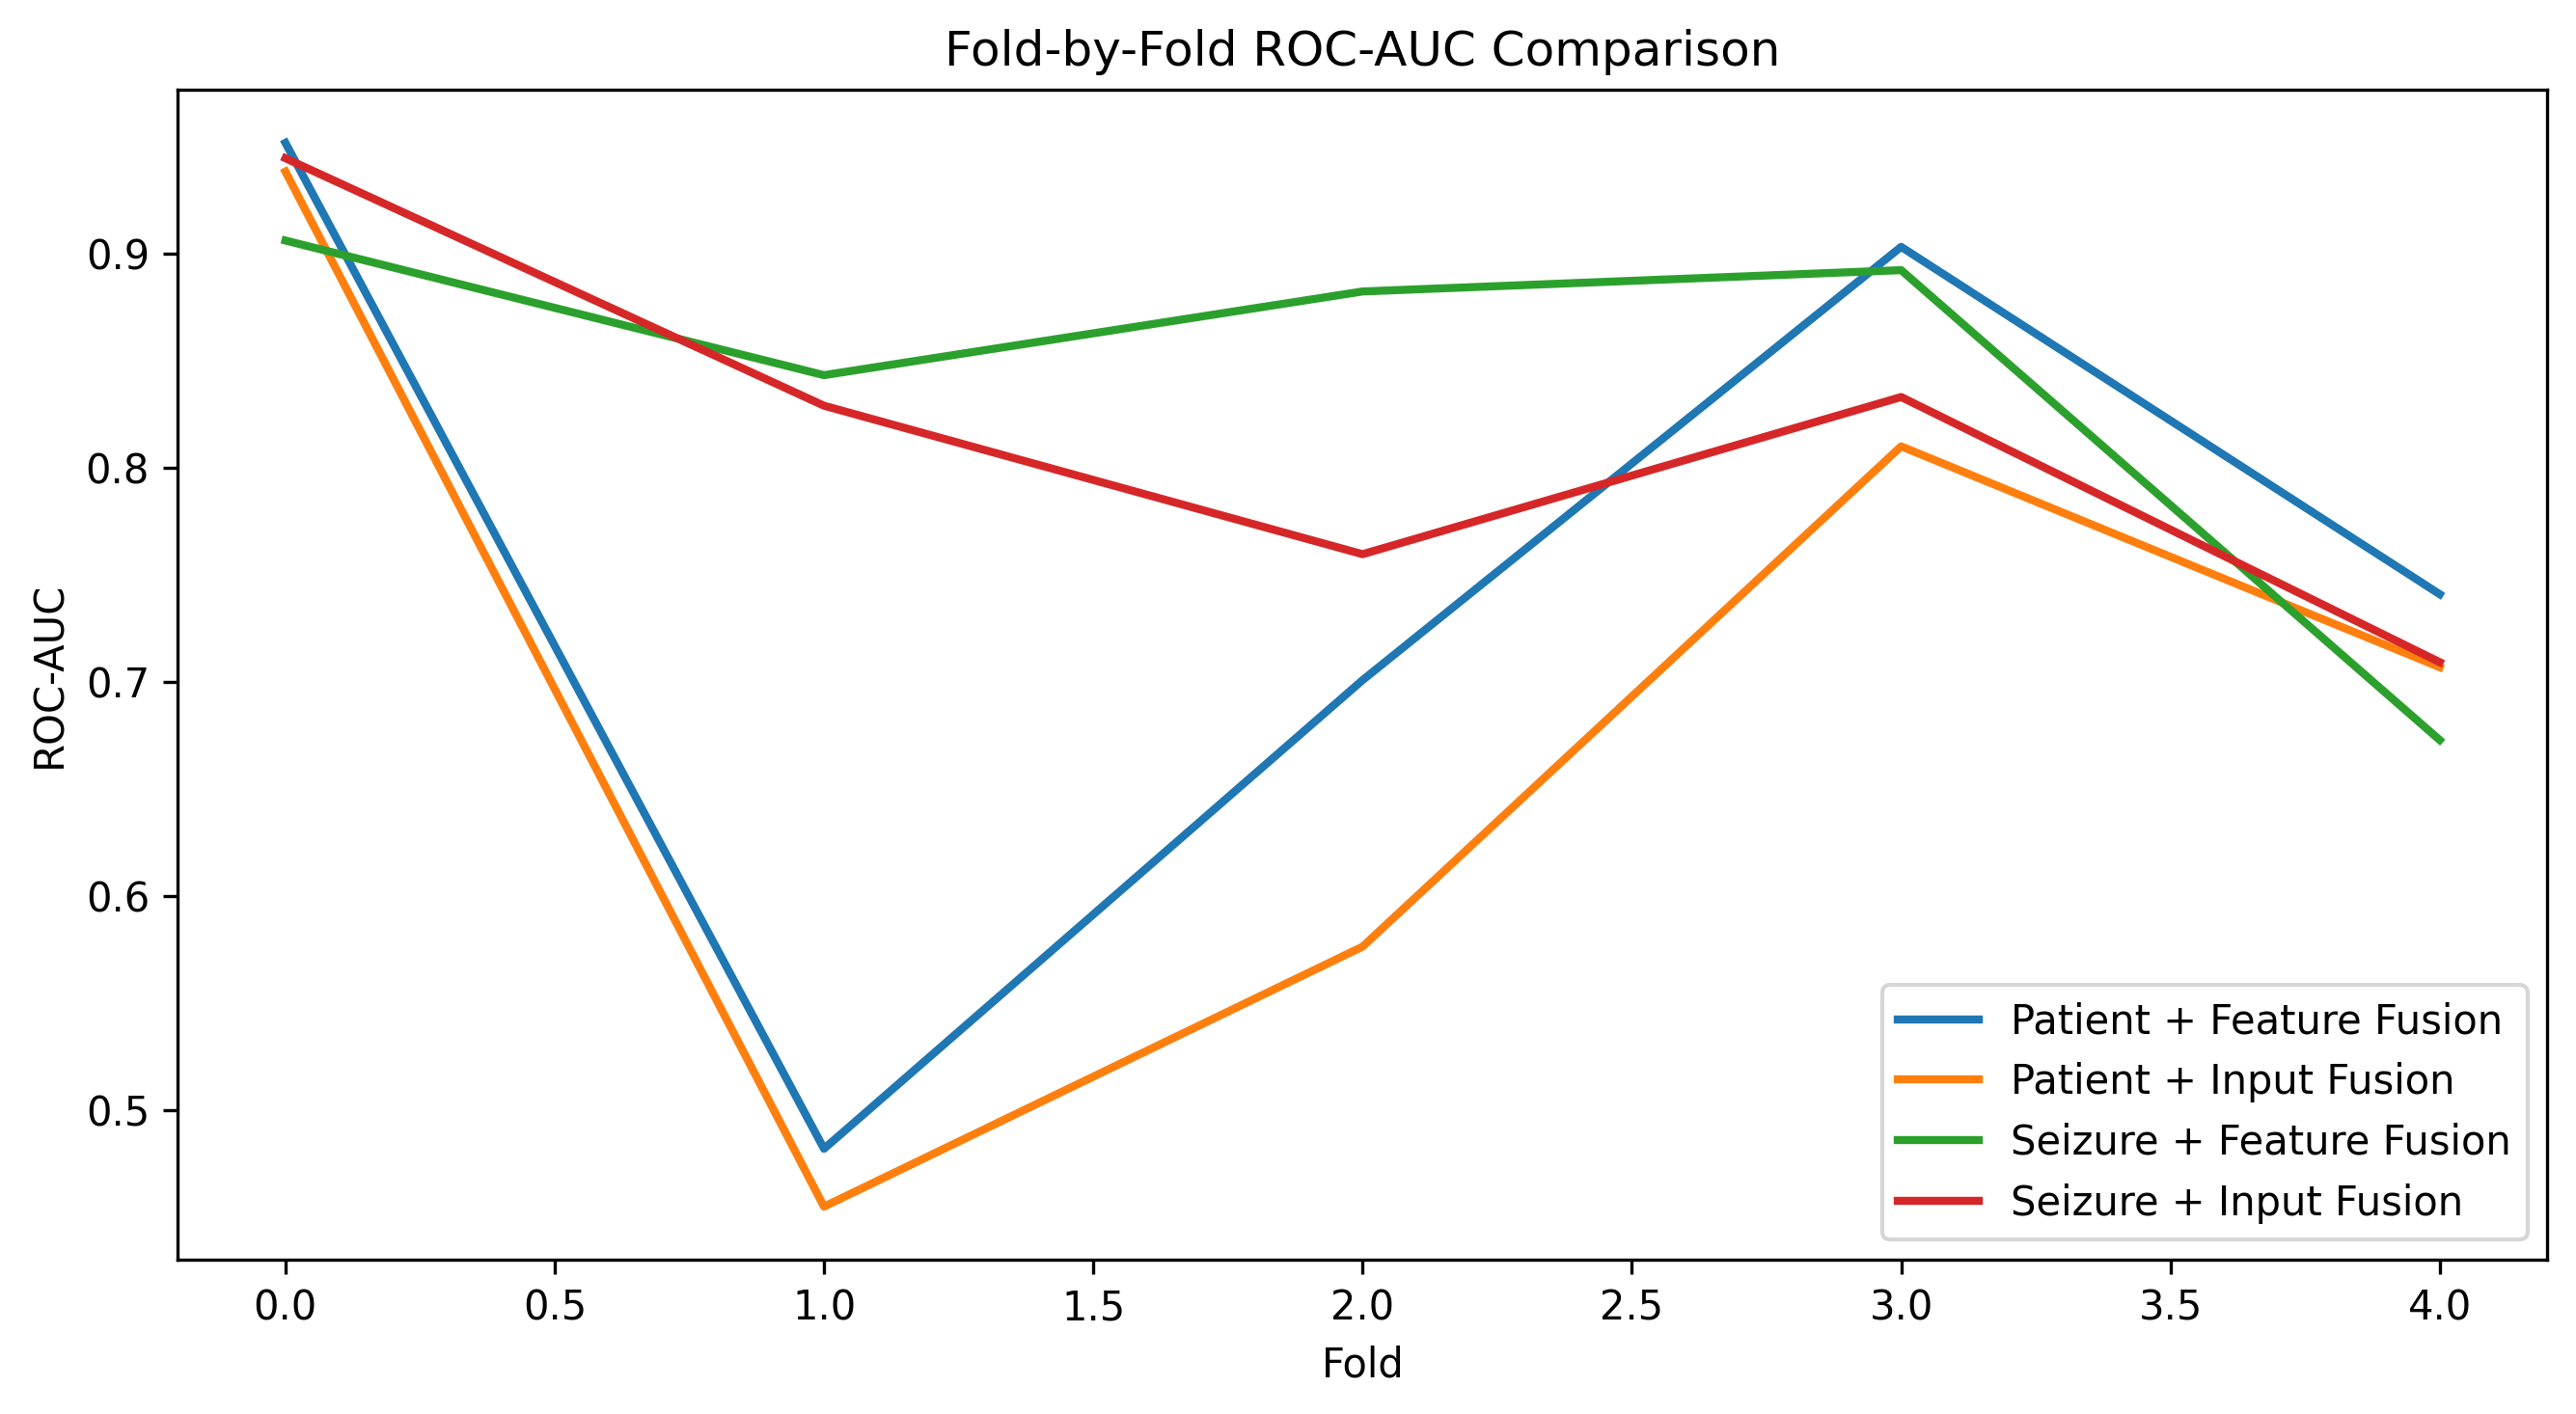
\includegraphics[width=0.88\textwidth]{generated_figures/Fig_03_foldwise_roc_auc.png}
    \caption{Fold-by-fold ROC-AUC comparison across all experiments.}
    \label{fig:foldwise_roc_auc}
\end{figure}

\begin{figure}[H]
    \centering
    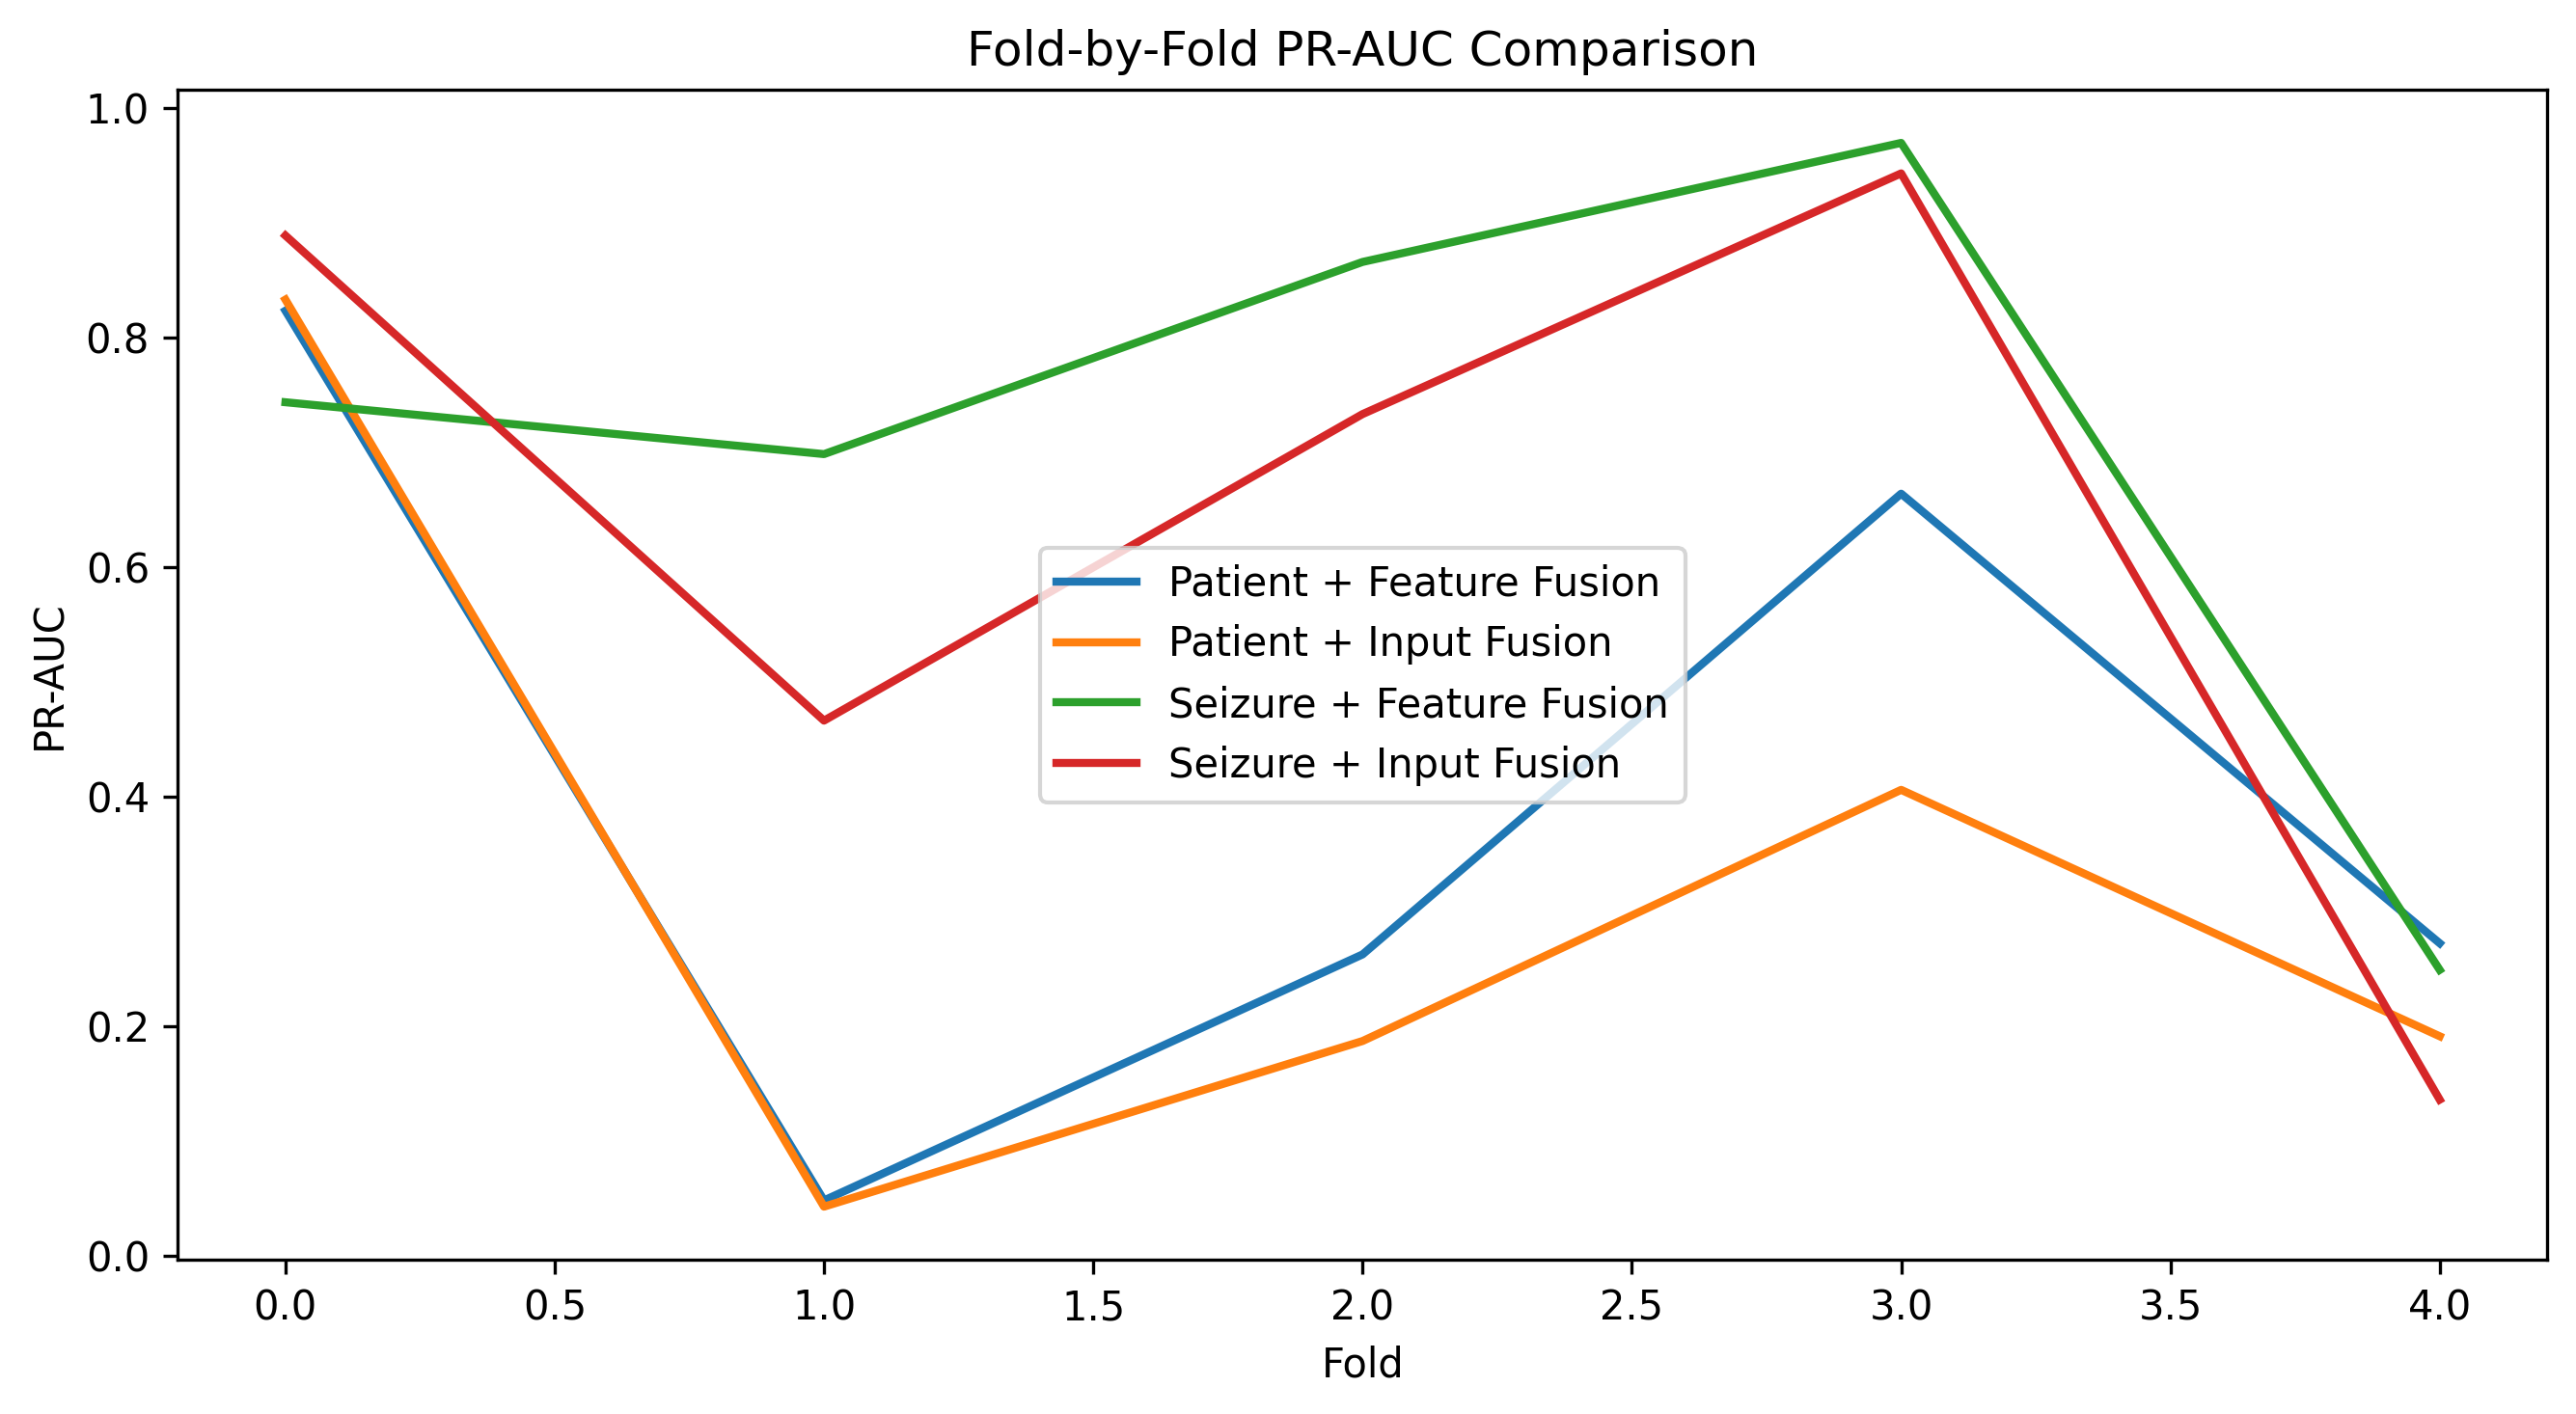
\includegraphics[width=0.88\textwidth]{generated_figures/Fig_04_foldwise_pr_auc.png}
    \caption{Fold-by-fold PR-AUC comparison across all experiments.}
    \label{fig:foldwise_pr_auc}
\end{figure}

\begin{figure}[H]
    \centering
    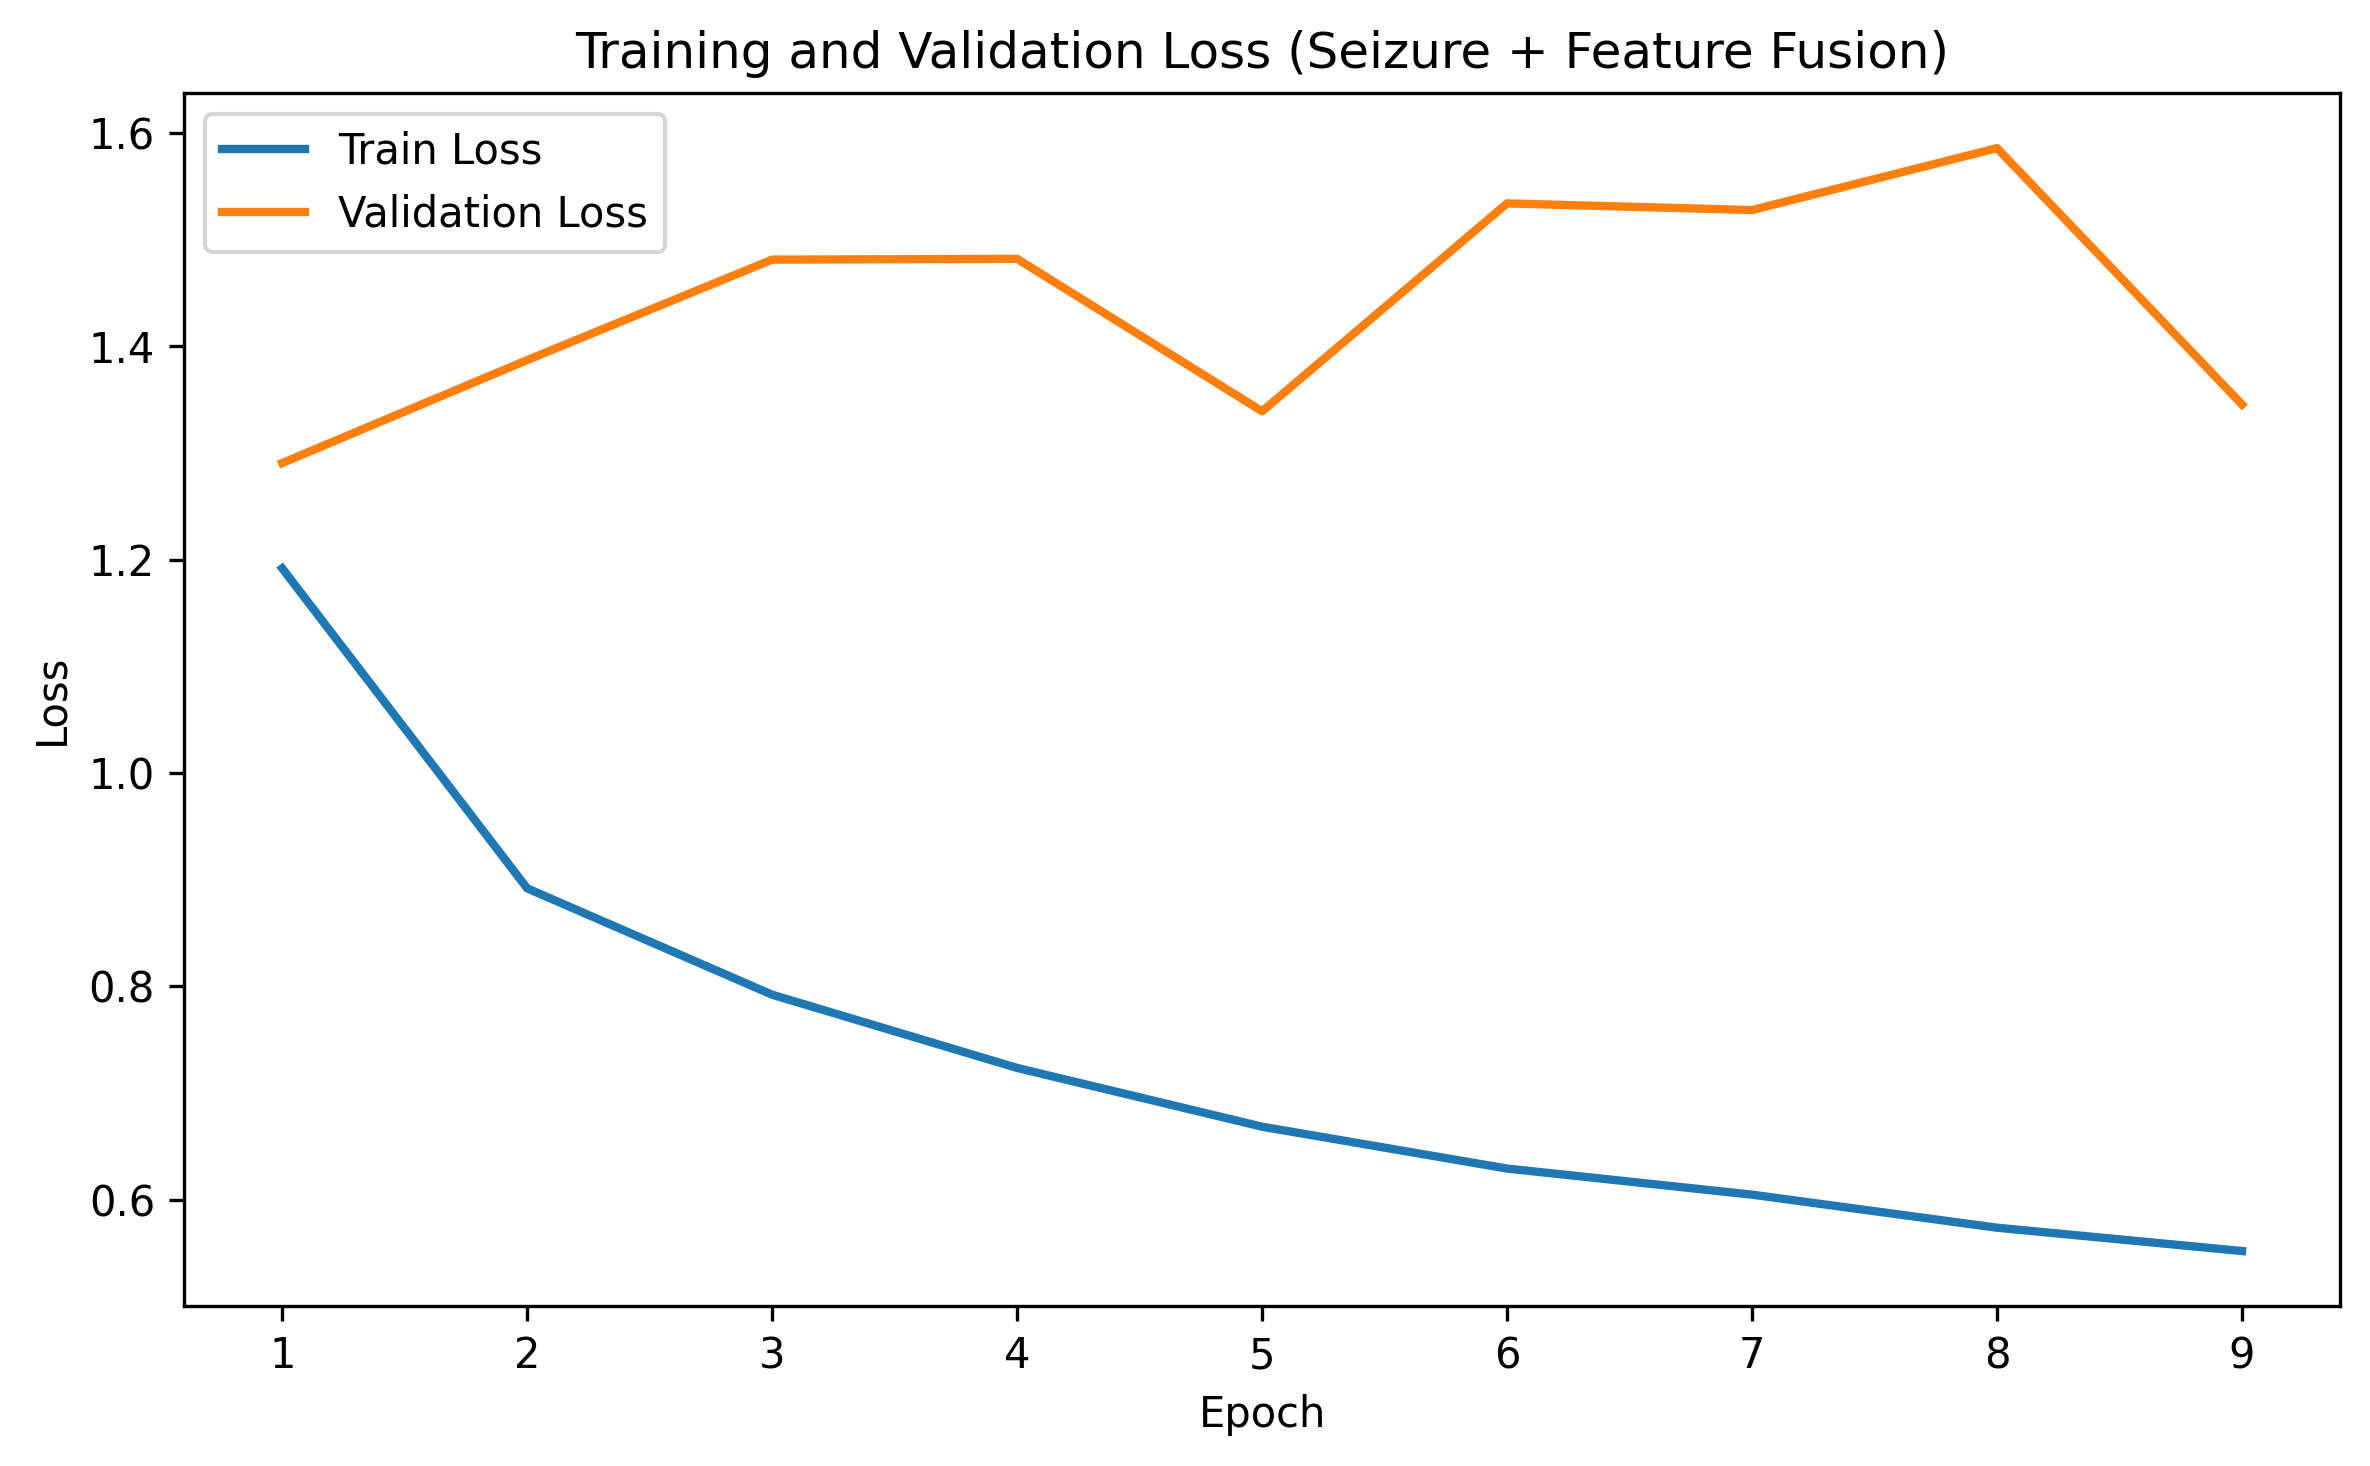
\includegraphics[width=0.88\textwidth]{generated_figures/Fig_05_seizure_feature_train_val_loss.png}
    \caption{Training and validation loss curves for a representative experiment fold.}
    \label{fig:train_val_loss}
\end{figure}

% Data table exported by the script: generated_figures/Table_02_mean_crossval_results.csv\n% Suggested caption: Mean cross-validation results.\n
% Data table exported by the script: generated_figures/Table_03_fold_by_fold_results.csv\n% Suggested caption: Fold-by-fold evaluation results for each experiment.\n
